\chapter{Measuring Local Sensitivity}

\begin{flushright}
\textit{A sensitivity index is a normalized derivative with a practical job.}

\medskip
\textit{Calibration tells you which parameter values fit the data.\\
Sensitivity analysis tells you which parameters matter to the answer.}
\end{flushright}

\bigskip

Two studies of the same epidemic model arrive at the following conclusions.

Study~A reports: ``Increasing the recovery rate by $1\%$ decreases $R_0$ by $1\%$.''

Study~B reports: ``Increasing the mean infectious period by $1\%$ increases $R_0$ by $1\%$.''

Both statements are mathematically correct. The recovery rate and
the mean infectious period are reciprocals of each other, so the
two studies analyzed the same model, used the same mathematics,
and obtained the same numerical result. Yet they convey opposite
signs and, more importantly, very different intuitions.
Study~A requires the reader to mentally invert a parameter before
the public health implication becomes clear.
Study~B is immediately interpretable: patients who are infectious
longer spread the disease more.

This chapter introduces the sensitivity index, the central
quantitative tool of this book, and develops the conventions
that make sensitivity analysis results readable rather than
merely correct.

%%------------------------------------------------------------
\section{Ratios as Precursors to Derivatives}
\label{sec:ratios}
%%------------------------------------------------------------

Comparison by ratio is one of the most fundamental quantitative
habits in applied science.
In finance, the price-to-earnings ratio tells an investor how many
dollars they pay for one dollar of profit.
In aeronautical engineering, the lift-to-drag ratio determines
whether a wing design is viable.
In experimental physics, the signal-to-noise ratio separates
measurement from artifact.
None of these ratios requires calculus. Each one gives a
dimensionless number that can be compared across different systems
and used to make decisions.

The sensitivity index is a ratio of this same type: it measures
how much the output changes, per unit change in the input,
normalized so that the result is dimensionless and comparable
across parameters with different units and scales.

To see why normalization matters, consider the price-to-earnings
ratio $P/E$. Suppose a stock trades at \$50 per share and has earned
\$2.50 over the past year. The $P/E$ ratio is $50/2.50 = 20$:
you pay \$20 for each dollar of annual earnings.
Now suppose earnings increase by $\$0.50$ to $\$3.00$.
A raw comparison of the two earnings figures gives $\$3.00 - \$2.50 = \$0.50$,
which tells you nothing useful without knowing the original value.
The normalized comparison is $(3.00 - 2.50)/2.50 = 20\%$, a
20\% increase in earnings, regardless of whether the numbers
are in dollars, euros, or any other currency.

A derivative, in the same spirit, measures the rate of change of
the output per unit change in the input. The sensitivity index
normalizes this derivative so that it answers a
specifically useful question: if the input changes by a small
percentage, by what percentage does the output change?

\begin{selfcheck}
A second stock trades at \$45 per share and has earned \$3.00 per year.
Calculate the $P/E$ ratio for each stock. Which stock is a better
value by this measure, and why?
\end{selfcheck}
\begin{scAnswer}
Stock~1: $P/E = 50/2.50 = 20$. Stock~2: $P/E = 45/3.00 = 15$.
Stock~2 has a lower $P/E$ ratio, meaning you pay less per dollar
of earnings, a better value by this measure.
The ratio provides a dimensionless comparison that is fair across
the two stocks despite their different prices and earnings.
\end{scAnswer}

%%------------------------------------------------------------
\section{Absolute, Relative, and Regularized Change}
\label{sec:change}
%%------------------------------------------------------------

Before defining the sensitivity index, we need precise language
for describing how quantities change. Three measures of change
appear throughout the book, each appropriate in different circumstances.

\subsection{Absolute Change}

Let $u$ denote the solution to a model, and suppose a perturbation
$\delta u$ is applied. The \textbf{absolute change} is simply the
difference between the perturbed and original solutions:
\begin{equation}
  \Dabs := \delta u = \hat{u} - u,
  \label{eq:abschange}
\end{equation}
where $\hat{u} = u + \delta u$ is the perturbed solution.
A 1-inch change in the length of a string has absolute change
1~inch, regardless of the original length.

\subsection{Relative Change}

The 1-inch change means something very different if the string is
6 inches long versus 1 mile long.
The \textbf{relative change}\index{relative change} accounts for this by normalizing against
the original value:
\begin{equation}
  \Drel := \frac{\delta u}{u} = \frac{\hat{u} - u}{u}.
  \label{eq:relchange}
\end{equation}
For the 6-inch string, the relative change is $1/6 \approx 16.7\%$.
For the 1-mile string ($63{,}360$ inches), it is $1/63{,}360 \approx 0.0016\%$.
The same absolute change has a very different significance depending
on context, and relative change captures this.

\subsection{Regularized Change}
\label{subsec:regularized}

Relative change has one practical problem: if $u \approx 0$,
the denominator in~\eqref{eq:relchange} is near zero and the
ratio becomes unreliable.
In dynamical models, the solution can pass through or near zero
during its evolution: the infectious compartment $I(t)$ in an epidemic
approaches zero as the outbreak resolves, for instance.
The \textbf{regularized change}\index{regularized change} handles this case by adding a
small correction to the denominator:
\begin{equation}
  \Dreg := \frac{\delta u}{1 + u}.
  \label{eq:regchange}
\end{equation}
When $u \approx 0$, this approximates absolute change: $\delta u / (1 + 0) = \delta u$.
When $u \gg 1$, it approximates relative change: $\delta u / (1 + u) \approx \delta u / u$.
The regularized change interpolates smoothly between the two regimes.

Looking more carefully at regularized change reveals a pattern that
recurs throughout applied mathematics: when a formula fails at a
special value, adding a small stabilizing term to the denominator
restores well-definedness without significantly changing the result
away from the problematic point. The same idea appears in numerical
linear algebra (Tikhonov regularization of ill-conditioned systems)
and in Bayesian statistics (pseudocounts in categorical models).
The regularized sensitivity index in Chapter~3 is one more instance.

\begin{selfcheck}
The infectious population in a disease model drops from $I = 0.04$
to $\hat{I} = 0.03$. Calculate the absolute, relative, and
regularized change. Which measure gives the most informative
description of this transition, and why?
\end{selfcheck}
\begin{scAnswer}
Absolute: $\delta I = 0.03 - 0.04 = -0.01$.
Relative: $-0.01/0.04 = -0.25$, a $25\%$ decrease.
Regularized: $-0.01/(1 + 0.04) \approx -0.0096$, close to absolute.

Since $I$ is small relative to 1, relative change gives the most
interpretable result: a $25\%$ decrease in the infectious population
is meaningful regardless of scale. For $I \ll 1$, absolute and
regularized change are both small in magnitude and harder to interpret
without the normalization that relative change provides.
\end{scAnswer}

%%------------------------------------------------------------
\section{The Sensitivity Index}
\label{sec:sensitivityindex}
%%------------------------------------------------------------

We now define the central tool of local sensitivity analysis.

\subsection{The Sign Rule}

Before any formal definition, the most important thing to know
about the sensitivity index is what its sign means.

\medskip
\noindent
\textbf{The sign rule:}\index{sign rule} A positive sensitivity index means that
the \QOI and \POI move in the same direction: increase the \POI
and the \QOI increases. A negative sensitivity index means they
move in opposite directions: increase the \POI and the \QOI
decreases. The magnitude tells you by how much: a sensitivity index
of $2$ means that a $1\%$ change in the \POI produces
approximately a $2\%$ change in the \QOI.

\medskip\noindent
\textbf{Important:} the sign belongs to the \emph{parameterization},
not to the underlying biology. The recovery rate $\gamma$ and the
mean infectious period $\tau = 1/\gamma$ describe the same biological
process, yet $\SI{\gamma}{R_0} < 0$ while $\SI{\tau}{R_0} > 0$.
When two papers report opposite signs for what appears to be the same
parameter, check whether they are using rate versus duration
parameterizations before concluding there is a contradiction.
Section~\ref{sec:interpretablePOIs} illustrates this with the SIR model.

\medskip

Students sometimes interpret a negative sensitivity index as
indicating an error in the calculation. It is not.
A negative index is often the best possible news: if the sensitivity
of $R_0$ with respect to the mean infectious period is positive, that
means longer illness leads to more transmission, and the corresponding
statement with the recovery rate would be negative: faster recovery
reduces transmission. Both facts are correct; the sign simply tells
you which direction the influence runs.
With this intuition established, the formal definition follows naturally.

\subsection{Formal Definition}

\begin{definition}[Sensitivity Index]\index{sensitivity index}
\label{def:SI}
Let $q$ denote a \QOI that depends differentiably on a \POI~$p$.
The \textbf{normalized sensitivity index}\index{sensitivity index!normalized} of $q$ with respect to $p$ is
\begin{equation}
  \SI{p}{q} := \lim_{\delta p \to 0}
               \frac{\left(\dfrac{\delta q}{q}\right)}
                    {\left(\dfrac{\delta p}{p}\right)}
             = \frac{p}{q}\,\frac{\partial q}{\partial p},
  \qquad q, p \neq 0.
  \label{eq:SI}
\end{equation}
\end{definition}

Three equivalent forms of this definition are in common use.
All three give the same number; which one is most convenient
depends on the problem at hand.

\textbf{Ratio form}\index{sensitivity index!ratio form} (Definition~\ref{def:SI}): the ratio of relative
changes in the \QOI and the \POI. This form is closest to the
P/E ratio analogy from Section~\ref{sec:ratios}.

\textbf{Derivative form}: multiply the partial derivative by the
ratio of nominal values:
\begin{equation}
  \SI{p}{q} = \frac{p}{q}\,\frac{\partial q}{\partial p}.
  \label{eq:SIderiv}
\end{equation}
This is the form used most often in computation.
The factor $p/q$ does the normalization work: it converts
$\partial q/\partial p$, which has units of $[Q]/[P]$ and depends
on the choice of units, into a dimensionless percent-for-percent ratio.
Concretely, if $\SI{p}{q} = 2$, then a $1\%$ increase in $p$
produces approximately a $2\%$ increase in $q$,
regardless of whether $p$ is measured in days, kilograms, or dollars.

\textbf{Logarithmic form}\index{sensitivity index!logarithmic form}: for positive \POIs and \QOIs,
\begin{equation}
  \SI{p}{q} = \frac{\partial \ln q}{\partial \ln p}.
  \label{eq:SIlog}
\end{equation}
This form reveals that the sensitivity index is the slope of the
log-log plot of $q$ versus $p$, a fact that becomes useful
when comparing SI values across very different scales.

The three forms are equivalent whenever $q$ and $p$ are
positive and $q$ is differentiable with respect to $p$.

\unifyingidea{1} The sensitivity index is the central object of this book.
It appears here as a ratio of relative changes. In Chapters~3 and 4
it reappears as a finite-difference approximation and as the solution
of a sensitivity equation. In Chapters~5 and 6, it appears as the
output of the adjoint calculation. In Chapter~9, it is the foundation
for Sobol variance decomposition. Every one of these is the same
normalized derivative, asked in the same way:
\emph{if the input changes by $x\%$, by what percentage does the output change?}

\medskip
\noindent\textbf{Why normalization is not optional.}\index{sensitivity index!dimensionlessness}
Without the $p/q$ factor, comparing raw derivatives across parameters
is not meaningful.
In the SIR model, $\partial R_0/\partial k$ has units of days
(since $k$ has units day$^{-1}$), while $\partial R_0/\partial \beta$
has different units entirely.
Asking which raw derivative is larger is like asking whether
1~pound is larger than 2~inches: the numbers may have any magnitude,
but the comparison is incommensurable because the units differ.
The normalized SI eliminates this problem.
Both $\SI{k}{R_0}$ and $\SI{\beta}{R_0}$ equal $+1$ --- dimensionless,
unit-free --- so ranking them is legitimate and the tornado plot
is an honest comparison.
This is why the tornado plot sorts by $|\SI{p}{q}|$ rather than
by $|\partial q/\partial p|$: only the normalized index gives
a ranking that is independent of how parameters happen to be measured.

\begin{selfcheck}
Use each of the three forms to compute the sensitivity index
of the area $A = \pi r^2$ with respect to the radius $r$.
Verify that all three give the same answer.
\end{selfcheck}
\begin{scAnswer}
\textit{Ratio form:} $\delta A / A = 2\pi r\,\delta r / (\pi r^2) = 2\delta r/r$,
so $\SI{r}{A} = (\delta A/A)/(\delta r/r) = 2$.

\textit{Derivative form:} $\partial A/\partial r = 2\pi r$, so
$\SI{r}{A} = (r/\pi r^2)(2\pi r) = 2$.

\textit{Logarithmic form:} $\ln A = \ln\pi + 2\ln r$, so
$\partial\ln A/\partial\ln r = 2$.

All three give $\SI{r}{A} = 2$: a $1\%$ increase in radius produces
a $2\%$ increase in area. The circle's area is twice as sensitive
to radius as to a parameter that appears linearly.
\end{scAnswer}

\subsection{Interpreting the Magnitude}
\label{subsec:magnitude}

The sensitivity index answers a specific quantitative question:
if the \POI changes by $x\%$, the \QOI changes by approximately $x \cdot \SI{p}{q}\%$.
For small $x$, this estimate is accurate to first order.
For larger $x$, second-order corrections become relevant, and
Chapter~3 discusses how to assess whether those corrections matter.

As a practical interpretive guide:
\begin{itemize}[nosep]
  \item $|\SI{p}{q}| > 1$: the \QOI is more sensitive than the \POI
        (the change in \QOI exceeds the change in \POI, percentage-for-percentage).
  \item $|\SI{p}{q}| = 1$: the \QOI changes in exact proportion to the \POI.
  \item $|\SI{p}{q}| < 1$: the \QOI is less sensitive than the \POI
        (the change in \QOI is smaller than the change in \POI).
  \item $|\SI{p}{q}| \approx 0$: the \QOI is essentially insensitive
        to this \POI near the nominal value.
\end{itemize}

%%------------------------------------------------------------
\section{Worked Examples}
\label{sec:workedexamples}
%%------------------------------------------------------------

The following examples build in complexity, beginning with
purely geometric functions and ending with the epidemic model
that serves as the book's primary running example.

\subsection{Volume of a Cylinder}
\label{subsec:cylinder}

The volume of a cylinder with radius $r$ and height $h$ is $V = \pi r^2 h$.
We want to know which dimension (radius or height)
has the greater effect on the volume.

Using the derivative form~\eqref{eq:SIderiv}:
\begin{equation}
  \SI{r}{V} = \frac{r}{V}\,\frac{\partial V}{\partial r}
            = \frac{r}{\pi r^2 h}\cdot 2\pi r h = 2.
  \label{eq:Vr}
\end{equation}
\begin{equation}
  \SI{h}{V} = \frac{h}{V}\,\frac{\partial V}{\partial h}
            = \frac{h}{\pi r^2 h}\cdot \pi r^2 = 1.
  \label{eq:Vh}
\end{equation}

The volume is twice as sensitive to radius as to height.
A $1\%$ increase in radius produces a $2\%$ increase in volume;
the same percentage increase in height produces only a $1\%$ increase.
This follows from the fact that $r$ appears squared in the volume formula
while $h$ appears linearly.

For a designer building a cylindrical tank with a fixed material budget,
this result has a direct implication: small manufacturing errors in the radius
matter twice as much as the same-sized errors in the height.

\begin{selfcheck}
For a cone with volume $V = \frac{1}{3}\pi r^2 h$, compute
$\SI{r}{V}$ and $\SI{h}{V}$. Compare with the cylinder results.
Explain why the answer is the same despite the different formula.
\end{selfcheck}
\begin{scAnswer}
$\SI{r}{V} = (r/V)(\partial V/\partial r) = (r/V)\cdot(2\pi r h/3) = 2$.
$\SI{h}{V} = 1$. Identical to the cylinder.

The reason: the sensitivity index depends on the \textit{exponent}
of each variable in the formula. Both $V_{\text{cone}} = \frac{1}{3}\pi r^2 h$
and $V_{\text{cylinder}} = \pi r^2 h$ have $r$ to the power $2$ and
$h$ to the power $1$. The constant $\frac{1}{3}$ cancels in the
logarithmic form $\partial\ln V/\partial\ln r = 2$. This is a
general principle: for a monomial $q = c\,p_1^{a_1}p_2^{a_2}\cdots$,
the sensitivity index with respect to $p_i$ is simply $a_i$.
\end{scAnswer}

\subsection{Arc Length of a Line}
\label{subsec:arclen}

Let $u(t) = mt + b$ be a line with slope $m$ and intercept $b$,
defined on $[0,a]$. The arc length is
\[
  J(m,b) = a\sqrt{1 + m^2}.
\]
Computing the sensitivity indices:
\begin{equation}
  \SI{m}{J} = \frac{m}{J}\,\frac{\partial J}{\partial m}
             = \frac{m}{a\sqrt{1+m^2}}\cdot\frac{am}{\sqrt{1+m^2}}
             = \frac{m^2}{1+m^2}.
\end{equation}
\begin{equation}
  \SI{b}{J} = \frac{b}{J}\,\frac{\partial J}{\partial b} = 0,
\end{equation}
since $J$ does not depend on $b$.

The arc length is completely insensitive to the intercept.
Geometrically, this is clear: shifting the line vertically does not
change its length. Analytically, $b$ does not appear in the formula
for $J$, so its derivative is zero. A zero sensitivity index is
not an error; it tells us that one \POI has no local effect
on the \QOI, which is itself an informative finding.

\begin{selfcheck}
For the line $u(t) = 3t + 2$ on $[0,4]$, compute $\SI{m}{J}$
numerically. Verify: if $m$ increases from $3$ to $3.03$ (a $1\%$ increase),
does $J$ change by approximately $\SI{m}{J}\%$?
\end{selfcheck}
\begin{scAnswer}
$\SI{m}{J} = m^2/(1+m^2) = 9/(1+9) = 0.9$.

At $m=3$: $J = 4\sqrt{10} \approx 12.649$.
At $m=3.03$: $J = 4\sqrt{1+3.03^2} = 4\sqrt{10.1809} \approx 12.763$.
Change: $(12.763 - 12.649)/12.649 \approx 0.90\% \approx 0.9 \times 1\%$. \checkmark
\end{scAnswer}

\subsection{Area Under a Line}
\label{subsec:area}

For the same line $u(t) = mt + b$ on $[0,a]$, the area is
\[
  J(m,b) = \int_0^a (mt + b)\,dt = \tfrac{1}{2}ma^2 + ba.
\]
Both parameters now affect the area:
\begin{equation}
  \SI{m}{J} = \frac{m}{\frac{1}{2}ma^2 + ba}\cdot\tfrac{1}{2}a^2
             = \frac{am}{am + 2b},
\end{equation}
\begin{equation}
  \SI{b}{J} = \frac{b}{\frac{1}{2}ma^2 + ba}\cdot a
             = \frac{2b}{am + 2b}.
\end{equation}
Note that $\SI{m}{J} + \SI{b}{J} = 1$, so the two indices
share a unit total for this particular linear functional.
This is not a general property: sensitivity indices do not
sum to any fixed value for arbitrary models or QOIs. Which parameter matters more depends on the
values: $\SI{m}{J} > \SI{b}{J}$ when $am > 2b$, and the
inequality reverses when $am < 2b$.

This example illustrates a general phenomenon: when two \POIs
both influence the same \QOI, their relative importance
depends on the nominal parameter values, not just on the
model structure. SA must always be reported at specific
nominal values.

\subsection{Root of a Nonlinear Equation}
\label{subsec:nonlinear}

Consider the nonlinear equation
\[
  f(u;\alpha) := \sin(\alpha u) - u = 0.
\]
For $\alpha = 2$, the equation has three roots;
for $\alpha > 1$, there is at least one nonzero root.
We want to know how the positive root $u^*(\alpha)$ changes
with $\alpha$.

Differentiating $f(u;\alpha) = 0$ implicitly with respect to $\alpha$:
\[
  u\cos(\alpha u) + \alpha\cos(\alpha u)\,\frac{\partial u}{\partial\alpha}
  - \frac{\partial u}{\partial\alpha} = 0.
\]
Solving for $\partial u/\partial\alpha$:
\[
  \frac{\partial u}{\partial\alpha}
  = \frac{u\cos(\alpha u)}{1 - \alpha\cos(\alpha u)}.
\]
At $\alpha = 2$, the positive root is $u^* \approx 0.9475$, giving
\[
  \SI{\alpha}{u^*}
  = \frac{\alpha}{u^*}\cdot\frac{u^*\cos(\alpha u^*)}{1 - \alpha\cos(\alpha u^*)}
  \approx -0.39.
\]
A $1\%$ increase in $\alpha$ decreases the positive root by approximately $0.39\%$.
This result requires no numerical experiment once the derivative is known;
the sensitivity index provides the estimate directly.

%%------------------------------------------------------------
\section{The Sensitivity Index for the SIR Model}
\label{sec:sirSI}
%%------------------------------------------------------------

The SIR epidemic model~\cite{kermack1927contribution,anderson1991infectious} describes the spread of an infectious disease
through a population divided into susceptible ($S$), infectious ($I$),
and recovered ($R$) compartments.
The basic reproduction number\index{basic reproduction number ($R_0$)}
\[
  R_0 = \frac{k\beta}{\gamma}
\]
measures the average number of new infections produced by one
infectious individual in an otherwise susceptible population,
where $k$ is the average number of contacts per day, $\beta$ is
the probability of transmission per contact, and $\gamma$ is the
recovery rate. The rigorous definition of $R_0$ via the next-generation
operator is given in van den Driessche and Watmough~\cite{vandendriessche2002reproduction}
and Diekmann et al.~\cite{diekmann1990definition}.

This is the book's primary running example.
In Chapter~4, we will compute time-dependent sensitivity indices
for the full SIR model. Here we compute the static sensitivity
indices for $R_0$: a closed-form calculation that introduces
all the key ideas in a familiar setting.

\subsection{Choosing Interpretable POIs}
\label{subsec:interpretable}

The parameters $k$, $\beta$, and $\gamma$ appear directly in the
model equations, which makes them a natural choice for \POIs.
However, we argued in Chapter~1 that \POIs should be chosen
to be interpretable in everyday terms.

The recovery rate $\gamma$ (units: day$^{-1}$) is not directly
interpretable. What a clinician understands and can measure is
the \emph{mean infectious period} $\tau = 1/\gamma$ (units: days):
the average number of days a patient remains infectious.
These two parameterizations are linked by:
\begin{equation}
  \SI{\tau}{q} = -\SI{\gamma}{q}
  \qquad\text{for any \QOI }q,
  \label{eq:reciprocalSI}
\end{equation}
since $\partial q/\partial\tau = (\partial q/\partial\gamma)
(\partial\gamma/\partial\tau) = -\gamma^2(\partial q/\partial\gamma)$,
giving $\SI{\tau}{q} = (\tau/q)(\partial q/\partial\tau)
= -(\gamma/q)\gamma(\partial q/\partial\gamma) = -\SI{\gamma}{q}$.

The magnitude is unchanged; the sign flips.
Table~\ref{tab:sirreparameterize} shows the effect of this
reparameterization for $R_0$.

\begin{table}[htb]
  \centering
  \begin{tabular}{llcc}
    \toprule
    \POI & Interpretation & Form & $\SI{p}{R_0}$ \\
    \midrule
    Recovery rate $\gamma$ (day$^{-1}$) & --- & rate & $-1$ \\
    Mean infectious period $\tau = 1/\gamma$ (days) & ``average days infectious'' & duration & $+1$ \\
    \midrule
    Contact rate $k$ (day$^{-1}$) & ``contacts per day'' & rate & $+1$ \\
    Transmission probability $\beta$ (dimensionless) & ``chance of infection per contact'' & probability & $+1$ \\
    \bottomrule
  \end{tabular}
  \caption{Sensitivity indices of $R_0$ with respect to rate and
           duration parameterizations of the SIR model.
           The mean infectious period $\tau = 1/\gamma$ has the same
           magnitude as $\gamma$ but opposite sign. The duration
           form is easier to interpret: a longer infectious period
           increases transmission, and both the sign and the
           plain-language statement agree.}
  \label{tab:sirreparameterize}
\end{table}

\subsection{Analytic Computation}
\label{subsec:R0SI}

With the interpretable \POIs $\{\tau = 1/\gamma,\, k,\, \beta\}$,
the sensitivity indices are:
\begin{align}
  \SI{k}{R_0} &= \frac{k}{R_0}\cdot\frac{\partial R_0}{\partial k}
                = \frac{k}{k\beta/\gamma}\cdot\frac{\beta}{\gamma} = 1,
                \label{eq:R0k} \\[4pt]
  \SI{\beta}{R_0} &= \frac{\beta}{R_0}\cdot\frac{\partial R_0}{\partial\beta}
                    = \frac{\beta}{k\beta/\gamma}\cdot\frac{k}{\gamma} = 1,
                    \label{eq:R0beta} \\[4pt]
  \SI{\tau}{R_0} &= -\SI{\gamma}{R_0}
                   = -\frac{\gamma}{R_0}\cdot\frac{\partial R_0}{\partial\gamma}
                   = -\frac{\gamma}{k\beta/\gamma}\cdot\left(\frac{-k\beta}{\gamma^2}\right) = +1.
                    \label{eq:R0tau}
\end{align}

All three \POIs have sensitivity index $+1$ with the interpretable
parameterization. In plain language: a $1\%$ increase in contact rate,
transmission probability, \emph{or} mean infectious period each
increases $R_0$ by $1\%$. The three parameters are equally important
for $R_0$, and all three promote disease spread when increased,
as every positive sign and every positive biological interpretation
confirms.

\begin{selfcheck}
An intervention reduces the contact rate $k$ by $20\%$.
Using the sensitivity indices above, estimate the change in $R_0$.
If a second intervention reduces the mean infectious period $\tau$
by $15\%$, which intervention has the greater effect on $R_0$?
\end{selfcheck}
\begin{scAnswer}
First intervention: $\Delta R_0/R_0 \approx \SI{k}{R_0}\times(-20\%) = -20\%$.
Second intervention: $\Delta R_0/R_0 \approx \SI{\tau}{R_0}\times(-15\%) = -15\%$.
The first intervention has the greater effect. Both indices equal $1$,
so the percentage change in $R_0$ equals the percentage change in the \POI.
The intervention that changes its \POI by the larger percentage
has the larger effect.
\end{scAnswer}

%%------------------------------------------------------------
\section{Choosing Interpretable POIs}
\label{sec:interpretablePOIs}
%%------------------------------------------------------------

The SIR example illustrates a general principle that should guide
every SA study before any calculation begins.

\textbf{Choose \POIs that can be discussed in ordinary language,
not merely because they appear in the model equations.}

Model equations are written in the language that is mathematically
convenient, which is not always the language that is scientifically
or operationally natural. Rates (with units day$^{-1}$) are
mathematically convenient in differential equations but not naturally
interpretable; the corresponding mean times (with units days)
are easier to discuss in a clinical or policy context.

The general rule for rate parameters in compartmental models:
if a parameter $p$ is a per-capita rate (units: time$^{-1}$),
define the corresponding \POI as $\tau = 1/p$ (the mean time
spent in that state), compute $\SI{\tau}{q} = -\SI{p}{q}$,
and report the result in terms of $\tau$.

Two additional cases arise frequently:

\textbf{Dimensionless probabilities.}
Transmission probabilities like $\beta$ are already dimensionless
and directly interpretable: ``a $25\%$ chance of transmission
per contact'' requires no conversion.

\textbf{Composite parameters.}
In the SIR model, $k$ and $\beta$ always appear together as the
product $k\beta$ in the expression for the force of infection
$\lambda = k\beta I/N$. Neither can be identified separately from
incidence data alone; only the product $k\beta$ is identifiable.
In this case, $k\beta$ is a more natural single \POI than either
factor individually. A related issue arises whenever two \POIs
are not independently changeable, which leads to the topic of
correlated \POIs in Chapter~3.

A practical check: if you cannot explain what a $1\%$ increase in a
\POI means in plain language to a colleague outside mathematics,
reconsider the parameterization.

It is worth noting that even in highly cited published work, this
distinction is sometimes overlooked.
Section~4.1 of Chitnis, Hyman \& Cushing~\cite{chitnis2008determining},
a paper that has become a standard reference for SA in mathematical
epidemiology, reports sensitivity indices using rate parameters
throughout. The SI values are mathematically correct, but several
indices are negative for parameters that clearly promote disease spread,
requiring a mental inversion before the public health interpretation
is clear. The present book recommends always asking, before reporting
any SI: would a policy maker understand this sign immediately,
or does it require translation?

One further misconception deserves attention here.
A sensitivity index near zero does \emph{not} mean a parameter is
globally unimportant. It means the model is approximately linear in
that parameter near the nominal value, and the linear term happens
to be small. If the model is nonlinear in that parameter, varying it
over a wider range may reveal substantial effects that the SI misses
entirely. Chapter~9 addresses this through global sensitivity analysis.

\begin{selfcheck}
A malaria model contains the parameter $\mu_v$ (mosquito mortality
rate, units: day$^{-1}$). A colleague reports $\SI{\mu_v}{R_0} = -0.3$.
Reparameterize in terms of mean mosquito lifespan $L = 1/\mu_v$
(units: days). What is $\SI{L}{R_0}$? Write a plain-language
interpretation of each sensitivity index.
\end{selfcheck}
\begin{scAnswer}
$\SI{L}{R_0} = -\SI{\mu_v}{R_0} = +0.3$.

Rate form: ``A $10\%$ increase in mosquito mortality rate decreases
$R_0$ by $3\%$.'' This requires mental inversion: higher mortality
$\to$ shorter lifespan $\to$ less transmission.

Duration form: ``A $10\%$ increase in mean mosquito lifespan increases
$R_0$ by $3\%$.'' Direct: longer-lived mosquitoes transmit more malaria.
\end{scAnswer}

%%------------------------------------------------------------
\section{The Tornado Plot}
\label{sec:tornadoplot}
%%------------------------------------------------------------

When a model has several \POIs, the collection of sensitivity indices
becomes a list of numbers with signs and magnitudes. Reading such a
list is manageable for three or four parameters; for ten or twenty,
a visual display is essential.

The \textbf{tornado plot}\index{tornado plot} is the standard display format for
sensitivity indices. It is a horizontal bar chart with the following
conventions:
\begin{itemize}[nosep]
  \item Bars extending to the \emph{right} indicate positive sensitivity
        indices (\POI and \QOI move in the same direction).
  \item Bars extending to the \emph{left} indicate negative sensitivity
        indices (opposite directions).
  \item Bars are sorted from largest to smallest by absolute magnitude,
        with the most influential parameter at the top.
  \item The length of each bar represents the magnitude of the index.
\end{itemize}
The sorted layout creates the ``tornado'' shape: wider at the top,
narrower toward the bottom.

Figure~\ref{fig:tornado_R0} shows the tornado plot for $R_0$
in the SIR model with \POIs $\{k, \beta, \tau\}$.
All three bars extend to the right (all indices are $+1$),
indicating that each parameter promotes disease spread when increased.
All bars are the same length, confirming that the three parameters
are equally important for $R_0$.

\begin{figure}[htb]
  \centering
  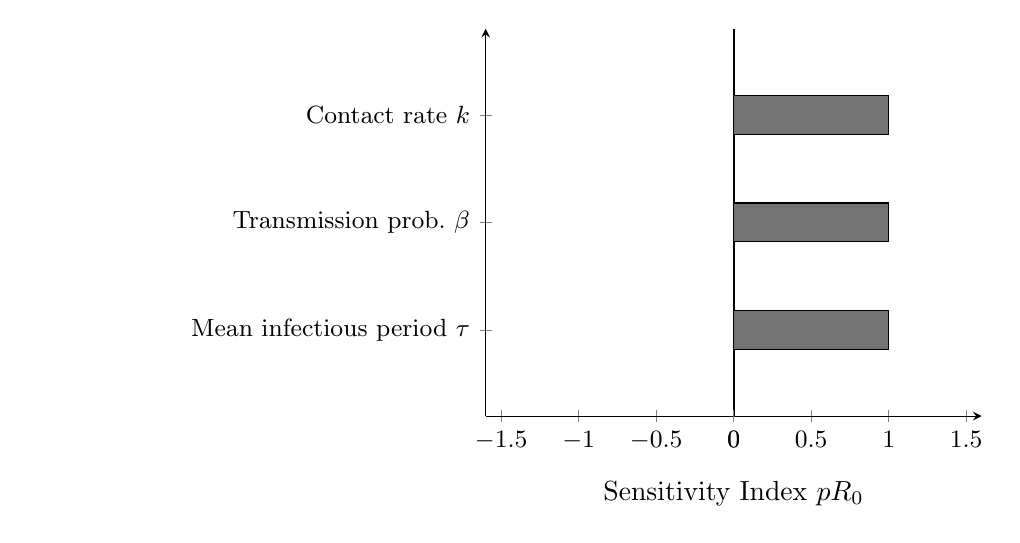
\begin{tikzpicture}
    \begin{axis}[
      xbar,
      bar width=14pt,
      width=0.65\textwidth,
      height=6.5cm,
      xmin=-1.6, xmax=1.6,
      xlabel={Sensitivity Index $\SI{p}{R_0}$},
      ytick={1,2,3},
      yticklabels={
        {Mean infectious period $\tau$},
        {Transmission prob.\ $\beta$},
        {Contact rate $k$}
      },
      yticklabel style={align=right, text width=5.5cm, font=\small},
      xticklabel style={font=\small},
      xtick={-1.5,-1,-0.5,0,0.5,1,1.5},
      extra x ticks={0},
      extra x tick style={grid=major, grid style={black, thick}},
      tick align=outside,
      axis x line=bottom,
      axis y line=left,
      enlarge y limits=0.4,
    ]
    \addplot[fill=black!55, draw=black] coordinates {
      (1,3)   %% k
      (1,2)   %% beta
      (1,1)   %% tau
    };
    \end{axis}
  \end{tikzpicture}
  \caption{Tornado plot for the sensitivity of $R_0$ to the three
           \POIs of the SIR model, parameterized using interpretable
           durations and probabilities. All three indices equal $+1$,
           so the bars are equal in length and all extend to the right.
           In models with more parameters and a wider range of index
           values, the sorted layout reveals immediately which
           parameters dominate.}
  \label{fig:tornado_R0}
\end{figure}

MATLAB code to produce a tornado plot for any set of sensitivity indices:

\begin{verbatim}
function tornado_plot(SI_values, labels, QOI_name)
% SI_values : vector of sensitivity indices
% labels    : cell array of POI names (strings)
% QOI_name  : string label for the QOI

[~, idx] = sort(abs(SI_values), 'descend');
SI_sorted  = SI_values(idx);
lab_sorted = labels(idx);

barh(SI_sorted, 'FaceColor', [0.35 0.35 0.35]);
set(gca, 'YTick', 1:numel(SI_sorted), ...
         'YTickLabel', lab_sorted, ...
         'FontSize', 11);
xline(0, 'k', 'LineWidth', 1.2);
xlabel(['Sensitivity Index  S_p^{' QOI_name '}'], 'FontSize', 12);
title(['Tornado Plot: Sensitivity of ' QOI_name], 'FontSize', 13);
grid on; box off;
end
\end{verbatim}

\begin{selfcheck}
A model for antibiotic-resistance spread has sensitivity indices
$\SI{\tau_{\mathrm{inf}}}{R_0} = +1.4$,
$\SI{\beta}{R_0} = +0.9$,
$\SI{\tau_{\mathrm{immune}}}{R_0} = -0.6$,
$\SI{k}{R_0} = +0.5$.

(a) Sketch the tornado plot by hand.
(b) Which parameter is most important? Least important?
(c) If $\tau_{\mathrm{immune}}$ (mean time spent immune) increases by $5\%$,
    what happens to $R_0$?
\end{selfcheck}
\begin{scAnswer}
(a) Sorted order by $|$SI$|$: $\tau_{\mathrm{inf}}$ ($1.4$, right),
$\beta$ ($0.9$, right), $\tau_{\mathrm{immune}}$ ($0.6$, \textit{left}),
$k$ ($0.5$, right).
(b) Most important: $\tau_{\mathrm{inf}}$. Least: $k$.
(c) $R_0$ decreases by approximately $0.6 \times 5\% = 3\%$.
The negative sign and the biological interpretation agree: a longer
immune period keeps people protected longer, reducing transmission.
\end{scAnswer}

%%------------------------------------------------------------
\section{A Preview: Second-Order Terms}
\label{sec:secondorder}
%%------------------------------------------------------------

The sensitivity index is built on a first-order approximation.
For a \QOI $q$ that depends on a single \POI $p$, the Taylor expansion gives
\[
  q(p + \delta p) = q(p)
    + \underbrace{\frac{\partial q}{\partial p}\,\delta p}_{\text{first-order}}
    + \underbrace{\frac{1}{2}\frac{\partial^2 q}{\partial p^2}\,(\delta p)^2}_{\text{second-order}}
    + \cdots
\]
The sensitivity index is derived from the first-order term alone.
When the second-order term is small relative to the first-order term
(that is, when
\[
  \left|\frac{1}{2}\frac{\partial^2 q}{\partial p^2}\,\delta p\right|
  \ll \left|\frac{\partial q}{\partial p}\right|,
\]
the sensitivity index provides an accurate approximation.
When this condition fails, the linear approximation is poor
and the SI overstates or understates the true sensitivity.

Chapter~3 develops practical methods for estimating the second-order
term numerically and for assessing when it is large enough to matter.
This is the first instance of Unifying Idea~3 from Chapter~1:
local SA is a linearization, and linearizations have limits.
The second-order term is the first correction beyond those limits.

For two \POIs $p_i$ and $p_j$ that are not varied independently
(a situation addressed in Chapter~3), the cross term
\[
  \frac{\partial^2 q}{\partial p_i\,\partial p_j}\,\delta p_i\,\delta p_j
\]
also enters the expansion. This cross derivative quantifies
the interaction between the two \POIs: it measures how the
sensitivity to $p_i$ changes as $p_j$ varies. Chapter~9 shows
how Sobol interaction indices generalize this idea to the full
range of parameter values.

%%------------------------------------------------------------
\section{MATLAB Laboratory: Sensitivity Indices for the SIR Model}
\label{sec:ch2matlab}
%%------------------------------------------------------------

This laboratory implements and visualizes the sensitivity indices
developed in the chapter, using the SIR model as the working example.
Complete the five parts in order; each builds on the previous.

\textbf{Part 1: Analytic SI via the Symbolic Toolbox.}
Define $R_0 = k\beta/\gamma$ symbolically in MATLAB.
Compute $\SI{k}{R_0}$, $\SI{\beta}{R_0}$, $\SI{\gamma}{R_0}$ using
the \texttt{diff} function and the derivative form of Definition~\ref{def:SI}.
Simplify and confirm that all three equal $\pm 1$ analytically.

\medskip\noindent
\textit{Note:} The code below requires the Symbolic Math Toolbox.
If you do not have it, skip directly to Part~3 and verify the same
results numerically. Parts~3--5 do not require the Symbolic Toolbox.

\begin{verbatim}
syms k beta gamma positive
R0   = k * beta / gamma;
SI_k = simplify( (k/R0) * diff(R0, k) )
SI_b = simplify( (beta/R0) * diff(R0, beta) )
SI_g = simplify( (gamma/R0) * diff(R0, gamma) )
\end{verbatim}

\textbf{Part 2: Reparameterize.}
Replace $\gamma$ with the mean infectious period $\tau = 1/\gamma$.
Rewrite $R_0 = k\beta\tau$ symbolically.
Compute $\SI{\tau}{R_0}$ and verify that it equals $-\SI{\gamma}{R_0}$
as predicted by equation~\eqref{eq:reciprocalSI}.

\textbf{Part 3: Numerical verification.}
Use the nominal values $k = 5$, $\beta = 0.06$, $\tau = 7$ days
(so $\gamma = 1/7$). Compute $R_0$ numerically. Estimate
$\SI{\tau}{R_0}$ using a centered finite difference with
$h = 10^{-5}\tau$. Compare with the analytic value of $+1$.
How large is the relative error?

\begin{verbatim}
k = 5; beta = 0.06; tau = 7;
R0    = k * beta * tau;
h     = 1e-5 * tau;
R0_p  = k * beta * (tau + h);
R0_m  = k * beta * (tau - h);
SI_fd = (tau / R0) * (R0_p - R0_m) / (2*h);
fprintf('Analytic SI: 1.00000\n');
fprintf('FD estimate: %.5f\n', SI_fd);
\end{verbatim}

\textbf{Part 4: Tornado plots for both parameterizations.}
Using the \texttt{tornado\_plot} function from Section~\ref{sec:tornadoplot},
produce two tornado plots side by side: one with rate parameters
$\{k, \beta, \gamma\}$ and one with interpretable parameters
$\{k, \beta, \tau\}$. Observe how the sign of the $\gamma/\tau$
bar changes between the two plots and why.

\medskip\noindent
\textit{MATLAB note:} The \texttt{tornado\_plot} function must be saved
as a separate file named \texttt{tornado\_plot.m} in your working directory
(function files cannot be pasted into a script).
Part~4 also uses \texttt{subplot} and cell array syntax for labels;
the file \texttt{run\_sir\_example.m} in the companion repository
demonstrates both if these are unfamiliar.

\textbf{Part 5: Effect of nominal value.}
Compute $\SI{k}{R_0}$, $\SI{\beta}{R_0}$, $\SI{\tau}{R_0}$ at
two different nominal transmission probabilities: $\beta_1 = 0.06$
and $\beta_2 = 0.6$. Do the SI values change? What does this
tell you about the sensitivity of $R_0$ to each parameter?
(Recall that $R_0 = k\beta\tau$ is a product of monomials;
for such functions, the SI is constant regardless of the nominal value.
This is a special property of multiplicative models that does not hold
for more complex functions like those in Chapter~4.)

%%------------------------------------------------------------
\section{Exercises}
\label{sec:ch2exercises}
%%------------------------------------------------------------

\begin{exercise}[\bloom{L2}]
\label{ex:ch2:signrule}
Explain the sign rule in your own words. Without performing any
calculation, state the sign of the sensitivity index for each of
the following, and explain your reasoning:
(a) the sensitivity of lung capacity to cigarette consumption,
    treating capacity as the \QOI and cigarettes per day as the \POI;
(b) the sensitivity of average crop yield to annual rainfall, near
    a region of the parameter space where crops are mildly drought-stressed;
(c) the sensitivity of $R_0$ to the mean infectious period $\tau$.
\end{exercise}

\begin{exercise}[\bloom{L2}]
\label{ex:ch2:threeforms}
For the function $q = \sqrt{p}$ (defined for $p > 0$), compute
$\SI{p}{q}$ using all three equivalent forms of Definition~\ref{def:SI}.
Verify that all three give the same result. Interpret the answer:
if $p$ doubles, by approximately what percentage does $q$ change?
\end{exercise}

\begin{exercise}[\bloom{L3}]
\label{ex:ch2:arcparabola}
Let $u(t) = \frac{1}{2}\lambda t^2$ be a parabola on $[0, b]$.
The arc-length functional is $J = \int_0^b \sqrt{1 + (\lambda t)^2}\,dt$.
Show that the sensitivity indices are
\[
  \SI{b}{J} = \frac{2\mu}{\mu + (\arcsinh\mu)/\sqrt{1+\mu^2}},
  \qquad
  \SI{\lambda}{J} = \frac{\mu(1+\mu^2) - \sqrt{1+\mu^2}\,\arcsinh\mu}
                        {\mu(1+\mu^2) + \sqrt{1+\mu^2}\,\arcsinh\mu},
\]
where $\mu = \lambda b$. For $\mu = 1$, compute both indices numerically
and verify using the derivative form.
\end{exercise}

\begin{exercise}[\bloom{L3}]
\label{ex:ch2:quadroots}
Let $u(t) = at^2 + bt + c$ and let $J_\pm = (-b \pm \sqrt{b^2 - 4ac})/(2a)$
denote the two real roots (assume $b^2 > 4ac$).
Show that the sensitivity indices of the positive root $J_+$ with respect to
$a$, $b$, $c$ can be written
\[
  \SI{a}{J_+} = -\frac{aJ_+}{2aJ_+ + b},
  \quad
  \SI{b}{J_+} = -\frac{b}{J_+(2aJ_+ + b)},
  \quad
  \SI{c}{J_+} = -\frac{c}{J_+(2aJ_+ + b)}.
\]
For $a=1$, $b=-3$, $c=2$, compute all three indices. Interpret each sign.
\end{exercise}

\begin{exercise}[\bloom{L3}]
\label{ex:ch2:SEIRR0}
A SEIR model (Susceptible-Exposed-Infectious-Recovered) has reproduction
number
\[
  R_0 = \frac{k\beta\,\nu}{(\nu + \mu)(\gamma + \mu)},
\]
where $\nu$ is the rate of progression from exposed to infectious,
$\mu$ is the background mortality rate, and $k$, $\beta$, $\gamma$
are as in the SIR model.
Reparameterize using mean times: $\tau_E = 1/\nu$ (mean latent period),
$\tau_I = 1/\gamma$ (mean infectious period), $L = 1/\mu$ (mean lifespan).
Compute $\SI{\tau_E}{R_0}$, $\SI{\tau_I}{R_0}$, $\SI{L}{R_0}$,
$\SI{k}{R_0}$, $\SI{\beta}{R_0}$ and produce a tornado plot.
Which parameter is most important?
\end{exercise}

\begin{exercise}[\bloom{L4}]
\label{ex:ch2:reparamjudge}
A published paper reports $\SI{\gamma}{R_0} = -1.0$ for an SIR model,
where $\gamma$ is the recovery rate in units of day$^{-1}$.
A second paper on the same model reports $\SI{\tau}{R_0} = +1.0$,
where $\tau = 1/\gamma$ is the mean infectious period in days.
A policy maker reading both papers is confused: one paper shows a
negative index, the other shows a positive index for what appears to
be the same parameter.

Write a one-paragraph explanation for the policy maker that
(a) resolves the apparent contradiction,
(b) explains which parameterization is more informative for policy,
and (c) describes what each sensitivity index means in plain language.
\end{exercise}

\begin{exercise}[\bloom{L4}]
\label{ex:ch2:tornado_interp}
The following tornado plot data is given for a food-safety model with
\QOI~$J =$ mean number of illness cases per outbreak. The sensitivity
indices are:
$\SI{\tau_c}{J} = +2.1$ (mean contamination duration, days),
$\SI{\beta_f}{J} = +1.8$ (food-to-person transmission probability),
$\SI{\tau_s}{J} = -1.3$ (mean hand-washing interval, days),
$\SI{k_f}{J} = +0.7$ (food contacts per day),
$\SI{\mu}{J} = -0.2$ (background clearance rate).
\begin{enumerate}[label=(\alph*)]
  \item Produce the tornado plot in MATLAB using the code template
        from Section~\ref{sec:tornadoplot}.
  \item Rank the five parameters by absolute importance.
  \item A public health program can achieve a $15\%$ reduction in either
        $\tau_c$ or a $20\%$ reduction in $k_f$. Which intervention
        reduces $J$ more? By how much?
  \item The parameter $\mu$ has a small negative index. Write a
        one-sentence interpretation of what this means for disease control.
\end{enumerate}
\end{exercise}

\begin{exercise}[\bloom{L5}]
\label{ex:ch2:studydesign}
You are advising the World Health Organization on a vaccine allocation
strategy for a new respiratory pathogen. A compartmental model has been
fitted to early outbreak data. The model has six parameters; their
sensitivity indices with respect to the \QOI ``total deaths at 6 months''
are not yet known.

Design the SA study. Your design should specify:
\begin{enumerate}[label=(\alph*)]
  \item Which parameterization you will use (rates or durations) for each
        parameter, and why.
  \item What \QOI or \QOIs you would compute sensitivity indices for,
        and what additional \QOI you might consider beyond the stated one.
  \item How you would present the results to a non-mathematical
        audience (what figure or table, and what the key message would be).
  \item One limitation of the local SA approach that the WHO advisors
        should be aware of in using these results.
\end{enumerate}
\end{exercise}

\begin{exercise}[\bloom{L6}]
\label{ex:ch2:critique}
A modeling study reports the following: ``Sensitivity analysis of
$R_0$ was performed with respect to all model parameters.
The parameters are listed in Table~3 using the standard model notation.
All sensitivity indices were positive, confirming that $R_0$ is
an increasing function of all model parameters.''

Table~3 lists recovery rate $\gamma$, mortality rate $\mu$, and
waning immunity rate $\rho$ alongside transmission and contact parameters.

Identify the error in the study's statement and explain specifically
what is wrong, referring to the mathematical relationship between
rates and their reciprocals. Restate the conclusion correctly.
\end{exercise}

%%------------------------------------------------------------

